\chapter{Introduction}
In his 1985 book, \emph{``Surely you're joking, Mr.\ Feynman!"}, the physicist Richard Feynman writes about an experience he had as a graduate student at Princeton University. One day, Feynman was scheduled to give a talk about his work at an ordinary weekly seminar, but the stars aligned to bring a host of famous names together into the audience for that week, including John von Neumann, Wolfgang Pauli, and Albert Einstein.
The story itself focuses on Feynman's understandable surprise and nervousness about the situation, but he also noted an interesting detail about these great minds --- they shared an uncanny ability to predict the outcomes of complex mathematical processes, without having to resort to using algebra to work through the equations by hand.

Feynman refers to this ability as being able to \emph{see} the physics, and was no doubt part of the inspiration behind \emph{Feynman diagrams}, an alternative representation of the complex equations that describe interactions between subatomic particles.

\pagebreak
For example, the equation
\begin{equation*}
  \definecolor{blue}{HTML}{0e5980}
  \definecolor{orange}{HTML}{ef5b00}
  \definecolor{purple}{HTML}{894189}
  \definecolor{yellow}{HTML}{808800}
  \mathcal{M} = 
  ({\color{blue}O_1} {\color{purple}ie\gamma^\mu}{\color{orange}I_1})
  \left({\color{yellow}\frac{-ig_{\mu\nu}}{p^2}}\right)
  ({\color{blue}O_2}{\color{purple}ie\gamma^\nu}{\color{orange}I_2})
\end{equation*}
and the Feynmann diagram
\begin{equation*}
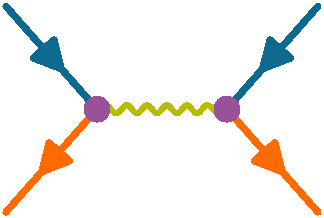
\includegraphics[width=.3\textwidth]{misc/feynman.pdf}
\end{equation*}
are equivalent, with both similarly colour-coded to match the corresponding elements of the interaction they are describing.
Both the equation and the diagram can be classified as a \emph{representations} of the abstract concept of a mathematical model, but it should be much clearer in the diagram that what is being described is the movement of two particles as they exchange a photon.

The subject of this thesis is not physics, so the details of the above interaction are not important. What is important is the fact that variations of these diagrams, with slightly different rotations and symbols, can closely approximate the behaviour of any subatomic particle interaction, whilst remaining simple enough to make complex and unwieldy integral expressions digestible. They helped open a door to understanding the natural world, revolutionising the field of quantum electrodynamics upon their introduction \cite{Kaiser2005}.
Feynman's contributions to science were eventually recognised by a Nobel prize shared with Shinichiro Tomonaga and Julian Schwinger, and the calculations behind their work could not have been possible without these diagrams \cite{Kaiser2009}.

% This is a beautiful example of \emph{visualisation} in work, and 
Why does this matter? Because the modern world has brought with it a powerful tool with the potential to further unlock this ability to \emph{see;}
not everybody can be a genius like Einstein or Feynman himself, but nowadays almost everybody does have access to something they did not: a personal computer.
% Computers have the power to show unprecedented amounts of information, with little delay from need to get. 
Tables of data no longer need to be plotted by hand, because a computer can do it automatically, without error, and on volumes of data impossible for any person to handle in multiple lifetimes.
But presenting this information in the best format to support human understanding is not trivial, because despite the brain's amazing ability for pattern recognition, it is also easily overloaded and often misled.
The study of what representations work best for humans, \emph{visualisation}, is the real subject of this thesis.

More specifically, the focus will centre upon on the visualisation of \emph{networks}. 
Any set of relationships between entities can be classified as a network. Commonly studied examples include networks of relationships on social media, biological metabolic pathways, and citation patterns between research publications. They can be found everywhere and are becoming an incredibly important data structure, but it is far from a trivial task to faithfully represent their underlying patterns, especially when the size of the network approaches the order of thousands or even millions of nodes. The majority of this thesis concerns the algorithms behind modern methods of network visualisation.

Another benefit of computers has been the development of user interfaces, which have flourished as a result of the massive recent growth in consumer electronics. This has brought a whole new language to the world, where people have learned the ability to communicate with machines, now small enough to carry in their pockets. There is a whole new generation of society who have grown up with these devices to become `computer-literate', granting them access to the world of \emph{interactive visualisation}, which dynamically responds to the user depending on what sections they wish to view, and how they wish to view them.
Despite this, static diagrams are still invaluable, not least because they can be printed on paper, which is still the most accessible form of media in the world. A well-organized static visualisation also allows the viewer to digest the information in their own time, and in the logical order that suits them best. This is just as a painting composed by a talented artist, with the right details spread across the right locations, can be observed and appreciated for just as long as a good movie.
As such, the majority of the work done here focuses on static visualisation. However it would be wasteful, if not foolish to ignore the wide realm of possibilities that interactive media can offer.

The final primary chapter of this thesis therefore explores an application of the algorithms developed in preceding chapters, in the form of a research-oriented video game called \emph{EcoBuilder}. Video games are, at their core, interactive visualisations with a single addition: there is an objective for the user/player to achieve through their actions. This goal in the context of EcoBuilder is to construct network of species connected by predator-prey interactions, whilst preventing any species from going extinct. The result of which species go extinct and which survive is determined by a dynamical system of equations used to model real-world ecosystems, and so the research outcome of the game is to crowdsource research into these dynamical systems through an approach known as \emph{citizen science}.

\section{Thesis roadmap}
This thesis is organised as follows. There are four main chapters, each of which explores a topic in the world of network visualisation. Chapter~\ref{chap:stress} concerns the layout of nodes in the node-link representation of a network. It presents the application of an algorithm known as stochastic gradient descent to the problem of node layout, which outperforms the previous state-of-the-art for a popular objective function known as stress.
Chapters~\ref{chap:heb} and~\ref{chap:power} concern the presentation of the links in a node-link diagram, specifically the idea of curving links to reduce clutter. Both chapters present methods that leverage the use of an auxiliary graph to inform this curvature.
The difference between the two chapters is the method for constructing this auxiliary graph: the first explored in Chapter~\ref{chap:heb} uses hierarchical clustering, and the second in Chapter~\ref{chap:power} uses power graph decomposition.
Chapter~\ref{chap:joy} presents an application of network visualisation algorithms to a research-oriented video game called EcoBuilder. A design study of the engineering challenges faced over its development is first presented, and the research outcomes from releasing the game to the public are then reported.

The broader literature review for the topics studied is split up across the chapters, in Sections~\ref{sec:nodes_background}, \ref{sec:edges_background}, and \ref{sec:joy_background}, each titled Background. A general context for the fields studied in this thesis as a whole can largely be garnered from reading each of the three individual chapters together, if desired. 
% However the thesis has been organised in a logical structure such that the text may be read in sequential order.
Overall conclusions are presented in the final Chapter~\ref{chap:conclusion} along with ideas for possible future work.

\section{Statement of Originality}
This is to certify that, to the best of my knowledge, the content of this thesis is my own work. This thesis has not been submitted for any other degree or other purposes.

I certify that the intellectual content of this thesis is the product of my own work and that all the assistance received in preparing this thesis and sources have been acknowledged.

\section{Publications}

The work in Chapter~\ref{sec:sgd} was previously published in Zheng et al.\ \cite{Zheng2019Stochastic}. The layout algorithm developed there was also applied to food webs in Ho et al.\ \cite{Ho2019}.
An early version of the work presented in Section~\ref{sec:heb_background} was previously published in Zheng et al.\ \cite{Zheng2018}
The work presented in Section~\ref{sec:power_graph} has previously been published in Zheng et al.\ \cite{Zheng2019Power}.
An early version of the game presented in Chapter~\ref{chap:joy} was published in Zheng et al.\ \cite{Zheng2019Eco}